\section{Example}
\label{sec:Example} 

In this section, we provide an example of the ETFT interface by depicting the core structure (i.e. finger tree) with internal vertices (i.e. sets) and sequences of pairs on the leaves (i.e. tours). Also, we illustrate the steps for computing \textit{split}s, \textit{insertion}s, \textit{concatenation}s, and lookups or \textit{view}s. All these the supporting functions to \textit{link} and \textit{cut} operations. Later, in Section~\ref{sec:TechDes}, we define these functions precisely describing their performance. 

\tcr{The whole section 3 is clumsy. Some of the pictures are useful to explain the idea of the annotations, but in many cases neither the text nor the figure add much information to what is already obviously from the name and type signature.}



Let us define two trees, $t_8$ and $t_2$. In this case we will consider the top vertex as the root, although, this is arbitrary and we can \textit{reroot} the tree at an existent vertex at any time.

Firstly, we have the tree $t_8$ on the left in in Figure~\ref{fig:t1et1ft1}, followed by its (only) Euler tour representation $et_8$ and its finger tree $ft_8$. At the top of $ft_8$ we have the monoidal representation of the set-union operation (shadowed ellipse) over all the leaf-vertices containing the pairs from $et_8$.
\begin{figure}
\begin{center}
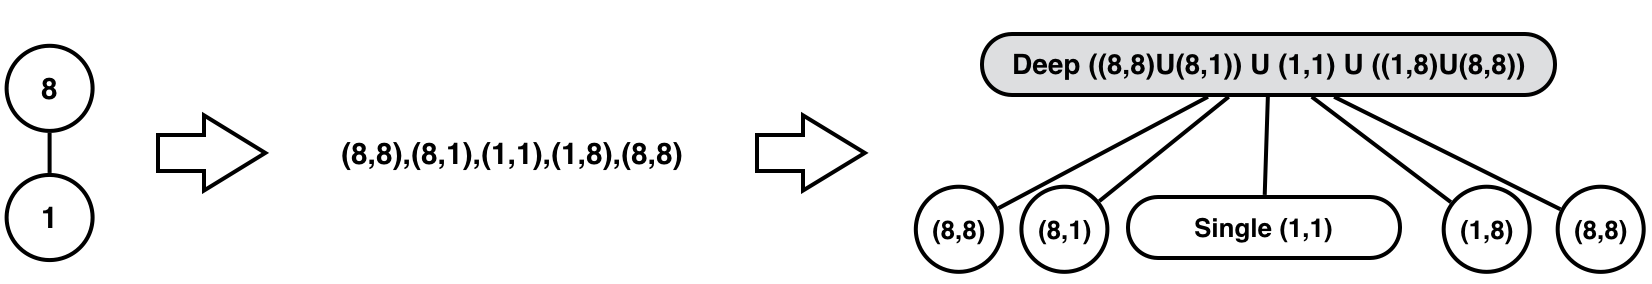
\includegraphics[scale=0.35]{./Images/t1et1ft1} 
\end{center}
\caption{Tree $t_8$ and its corresponding Euler tour $et_8$ and finger tree $ft_8$}
\label{fig:t1et1ft1}
\end{figure}

As an second example, we have $t_2$, Figure~\ref{fig:t2et2ft2}. The spine of the finger tree now contains a \code{Single} type constructor altogether with a \code{Node3}. Again, shadowed ellipses refer to the monoidal annotations \code{Set} where the set-insertion and set-union take place \textit{automatically}.
\begin{figure}
\begin{center}
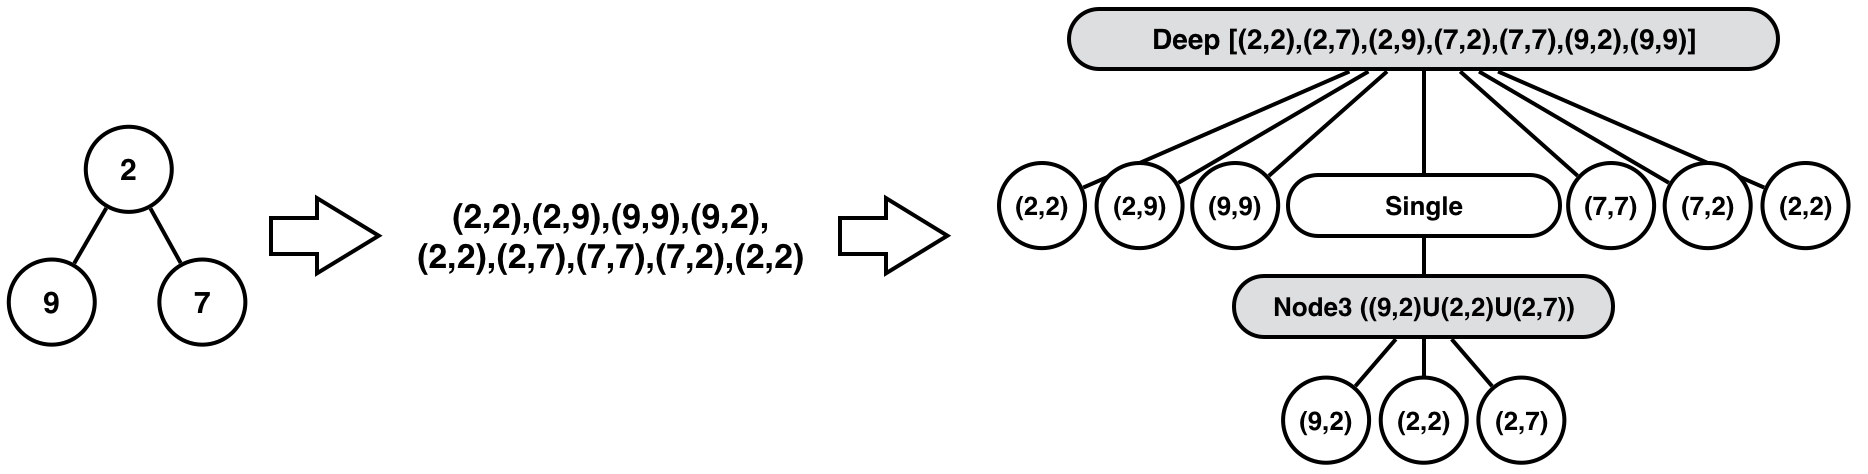
\includegraphics[scale=0.35]{./Images/t2et2ft2} 
\end{center}
\caption{Tree $t_2$ and its corresponding Euler tour $et_2$ and finger tree $ft_2$}
\label{fig:t2et2ft2}
\end{figure}

Now, the forest $f$ in Figure~\ref{fig:forest} is formed by inserting $ft_8$ and $ft_2$ from left and right respectively, in $O(1)$. The forest's \code{Deep} type constructor has the set-union of all the finger trees ($ft_8$ and $ft_2$), depicted in back colour with white font. The thick lines coming out from the top ellipse are the components of the top finger tree: two \code{Digit} and an \code{Empty} subtree (or subforest).
\begin{figure}
\begin{center}
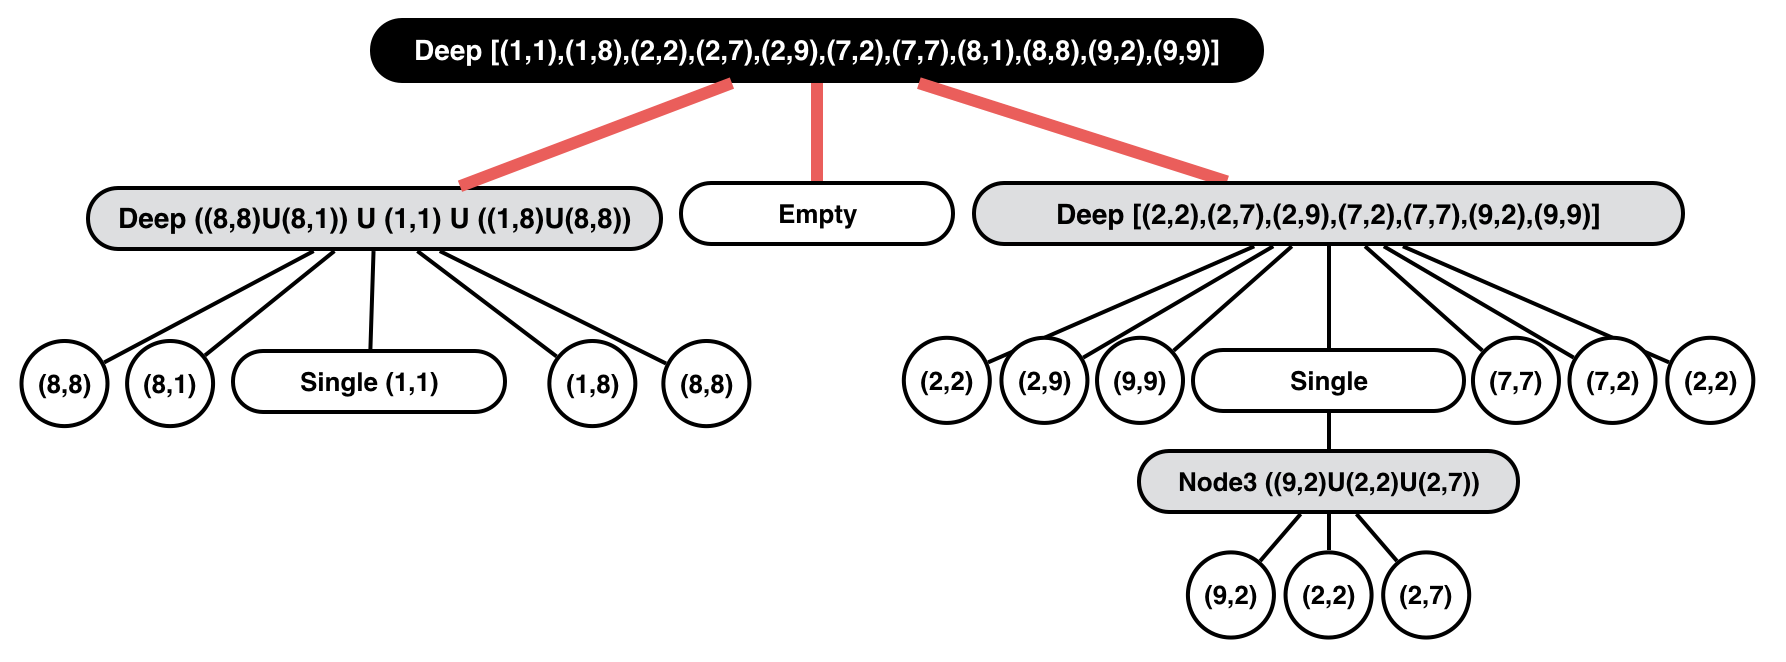
\includegraphics[scale=0.35]{./Images/forest} 
\end{center}
\caption{The forest $f$ comprising finger trees (Euler tours) as elements}
\label{fig:forest}
\end{figure}

Following, we have the basic operations for dynamic trees. Left side of Figure~\ref{fig:rootReroot} shows the \code{root} of a tree $t$ returning a vertex $v$, which is the first element of its finger tree $ft$, implemented in \code{viewl}. Rerooting a tree, by calling \code{reroot}, ask for a vertex $v$ and returns a \textit{new} tree. This is depicted in right side of Figure~\ref{fig:rootReroot}. This operation involves split, concatenation and insertions detailed in Section~\ref{sec:TechDes}.
\begin{figure}
\begin{center}
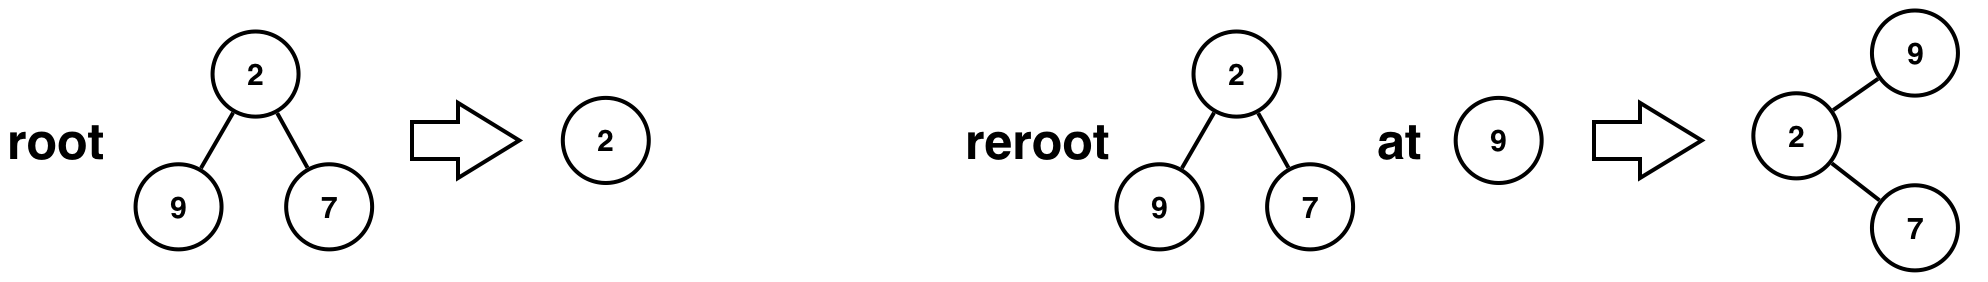
\includegraphics[scale=0.3]{./Images/rootReroot} 
\end{center}
\caption{\textit{root} and \textit{reroot} of a tree}
\label{fig:rootReroot}
\end{figure}

Splitting a finger tree, \code{split}, returns two subtrees (i.e. left and right) and an element, either a pair or an Euler tour, depending on the top container, a tree or a forest. This is depicted in Figure~\ref{fig:split}.
\begin{figure}
\begin{center}
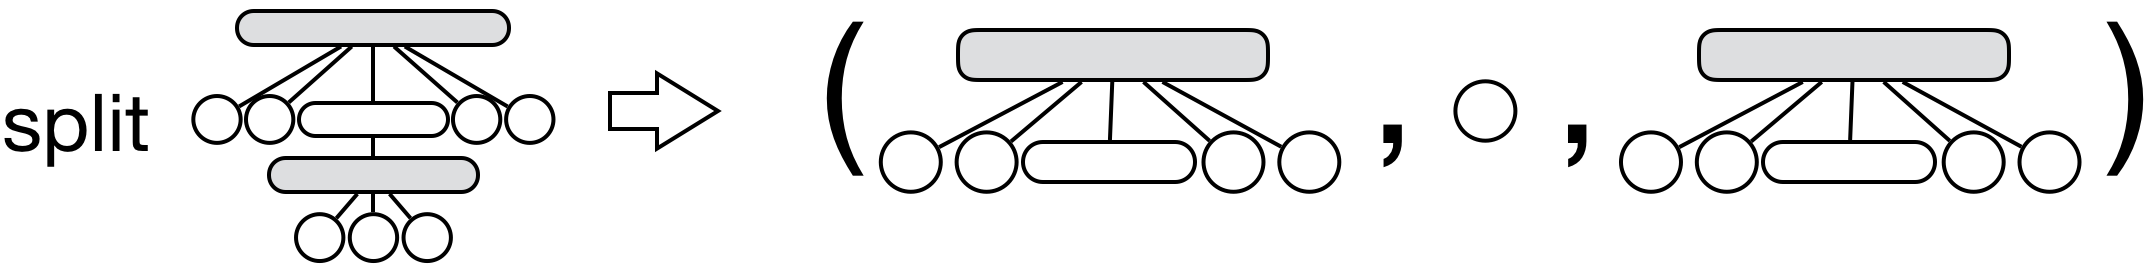
\includegraphics[scale=0.25]{./Images/split} 
\end{center}
\caption{Splitting a tree returns two smaller trees altogether an element}
\label{fig:split}
\end{figure}

Concatenating (also called appending) takes two finger trees and returns another (bigger) finger tree, as in Figure~\ref{fig:concatenation} and its represented by the $\bowtie$ symbol.
\begin{figure}
\begin{center}
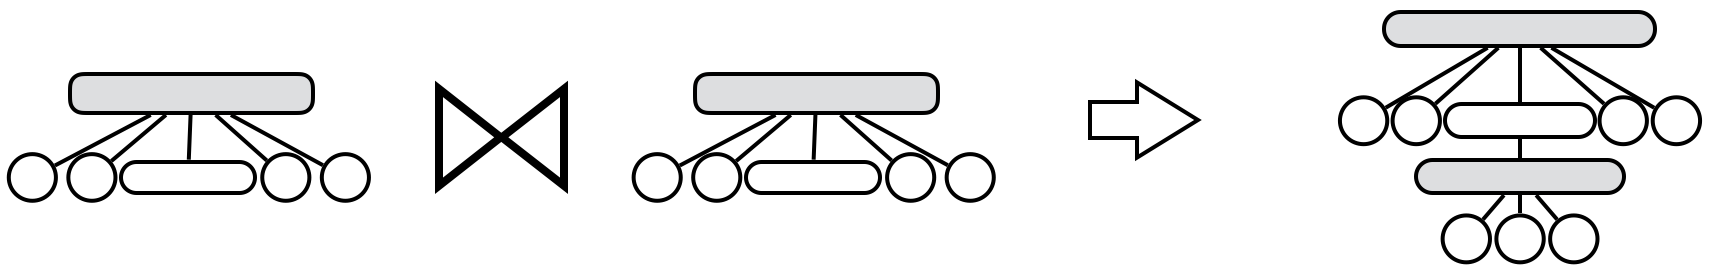
\includegraphics[scale=0.25]{./Images/concatenation} 
\end{center}
\caption{Concatenating two trees, returns a new one bigger}
\label{fig:concatenation}
\end{figure}


\tcr{Since the split operation over finger trees is central to the code, the paper would benefit from a more thorough explanation than the current incomplete type signatures (Concretely I'm missing an explanation of split's two first arguments).}


\tcr{The paper heavily builds on finger trees and tries to explain what they are and how they work, but omit aspects that are crucial to the understanding of the paper. In particular the `split` function is not explained, only listed in Table 2, but used in almost every listing later in the paper. The type listed for `split` mentions an unexplained type constructor `Split` and its type does not match the uses of `split`. The explanation around Fig. 5 does not help. What are the two first arguments to `split`?}




Under Figure~\ref{fig:consleftsnocright} we depict the final four help-functions that support \textit{link} and \textit{cut}: \code{viewl}, $\lhd$ (or \textit{cons}), $\rhd$ (or \textit{snoc}) and \textit{viewr}.
\begin{figure}
\begin{center}
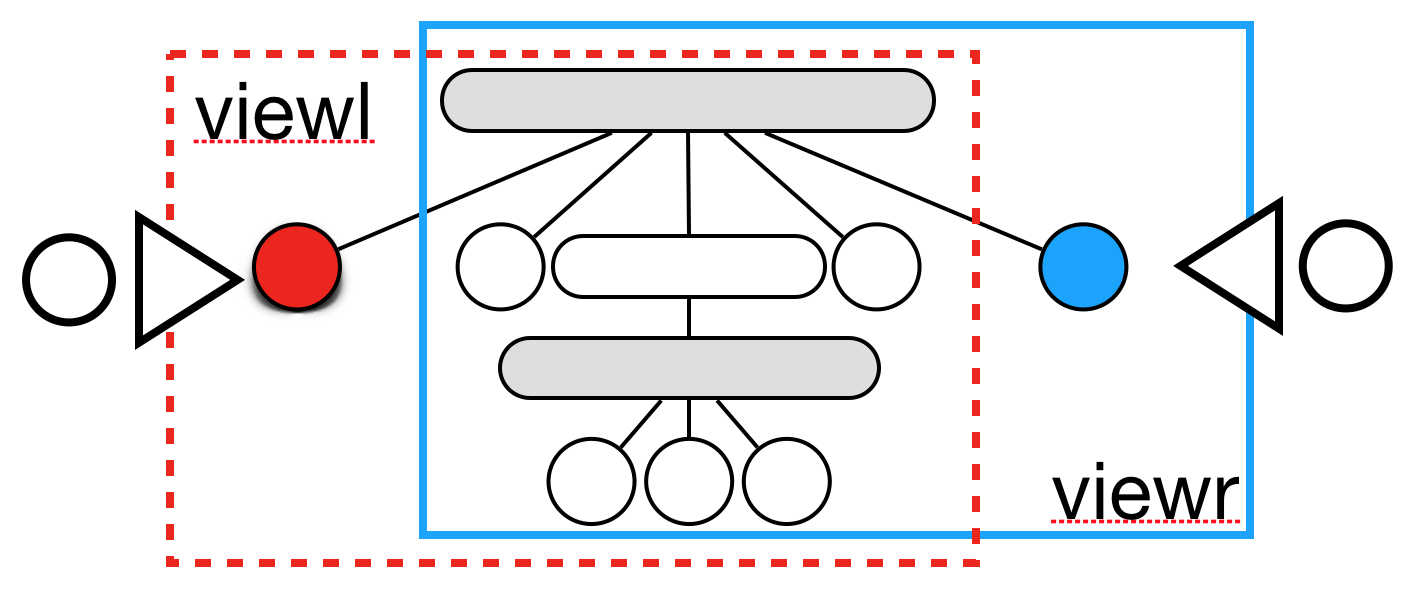
\includegraphics[scale=0.25]{./Images/consleftsnocright} 
\end{center}
\caption{Inserting and viewing from left (\code{viewl},$\lhd$) and inserting and viewing from right (\code{viewr},$\rhd$) }
\label{fig:consleftsnocright}
\end{figure}






